\documentclass[a4paper, twoside]{article}
\setcounter{secnumdepth}{5}
\setcounter{tocdepth}{5}
\usepackage[english]{babel}
\usepackage{textcomp}
\usepackage{amsmath,amsthm,amsfonts,amssymb,epsfig}
\usepackage{array}
\usepackage{datetime}
\usepackage{lipsum}% http://ctan.org/pkg/lipsum
\usepackage[left=1.1in,top=1in,right=1.1in]{geometry}% http://ctan.org/pkg/geometry
\usepackage{listings}% http://ctan.org/pkg/listings
\usepackage{spverbatim}
\usepackage{hyperref}
\usepackage{microtype}
\hypersetup{colorlinks=true, urlcolor=black, linkcolor=black}
\usepackage{graphicx}
\graphicspath{ {images/} }
\usepackage{parskip}
\usepackage{titlesec} %used for diminishing heading sizes
\usepackage[square, sort, comma, numbers]{natbib} %%uses titles for cited references
\usepackage[fit]{truncate}
\usepackage{fancyhdr}
\pagestyle{fancy}
\fancyhead{}
\fancyhead[RO, RE]{\thepage}
\fancyhead[LO, LE]{\rightmark}
\renewcommand{\sectionmark}[1]{\markboth{}{\textsc{\thesection~#1}}}
\fancyfoot[C]{}%hide footer
\usepackage{xcolor} 
\usepackage[scaled=1]{couriers}

\xdefinecolor{gray}{rgb}{0.6,0.6,0.6} 


\titleformat*{\section}{\LARGE\bfseries\sffamily}
\titleformat*{\subsection}{\Large\bfseries\sffamily}
\titleformat*{\subsubsection}{\large\bfseries\sffamily}
\titleformat*{\paragraph}{\large\bfseries\sffamily}
\titleformat*{\subparagraph}{\large\bfseries\sffamily}
\renewcommand{\familydefault}{\sfdefault} %sans-serif font


%
% Use fancy table
%
\usepackage{tabularx}
\usepackage{booktabs}

\begin{document}


%----------------------------------------------------------------------
% Definition for "lstlisting" blocks
%----------------------------------------------------------------------
% --- USAGE ---
%
% \begin{lstlisting}[style=R}
% ...
% \end{lstlisting}
%
% % \begin{lstlisting}[style=output}
% ...
% \end{lstlisting}
%----------------------------------------------------------------------

% By default, make listings all black so it's easy to spot the ones that aren't set to a style.
% This is just a debugging technique.
\lstset{backgroundcolor=\color{black}}

% Define scala language first
% ``define'' Scala
\lstdefinelanguage{scala}{
  morekeywords={abstract,case,catch,class,def,%
    do,else,extends,false,final,finally,%
    for,if,implicit,import,match,mixin,%
    new,null,object,override,package,%
    private,protected,requires,return,sealed,%
    super,this,throw,trait,true,try,%
    type,val,var,while,with,yield},
  otherkeywords={=>,<-,<\%,<:,>:,\#,@},
  sensitive=true,
  morecomment=[l]{//},
  morecomment=[n]{/*}{*/},
  morestring=[b]``,
  morestring=[b]',
  morestring=[b]''``
}

\lstdefinestyle{R}{
  language=R,
  frame=single,
  breaklines,
  basicstyle=\ttfamily,
  commentstyle=\textbf,% comment style
  keywordstyle=\ttfamily,
  numbers=left,% display line numbers on the left side 
  numberstyle=\scriptsize,% use small line numbers 
  numbersep=10pt,% space between line numbers and code
  backgroundcolor=\color{white}, 
  showstringspaces=false % don't show spaces as weird char.
}

\lstdefinestyle{python}{
  language=python,
  frame=single,
  breaklines,
  basicstyle=\ttfamily,
  commentstyle=\textsl,% comment style
  keywordstyle=\ttfamily,
  numbers=left,% display line numbers on the left side 
  numberstyle=\scriptsize,% use small line numbers 
  numbersep=10pt,% space between line numbers and code
  backgroundcolor=\color{white}, 
  showstringspaces=false %don't show spaces as weird char.
}

\lstdefinestyle{Scala}{
  language=scala,
  frame=single,
  breaklines,
  basicstyle=\ttfamily,
  commentstyle=\textsl,% comment style
  keywordstyle=\ttfamily,
  numbers=left,% display line numbers on the left side 
  numberstyle=\scriptsize,% use small line numbers 
  numbersep=10pt,% space between line numbers and code
  backgroundcolor=\color{white}, 
  showstringspaces=false % don't show spaces as weird char.
}

\lstdefinestyle{Bash}{
  language=bash,
  frame=single,
  breaklines,
  basicstyle=\ttfamily,
  commentstyle=\textsl,% comment style
  keywordstyle=\ttfamily,
  numbers=left,% display line numbers on the left side 
  numberstyle=\scriptsize,% use small line numbers 
  numbersep=10pt,% space between line numbers and code
  backgroundcolor=\color{white}, 
  showstringspaces=false % don't show spaces as weird char.
}


\definecolor{mygray}{rgb}{0.92,0.92,0.92}

\lstdefinestyle{output}{
  frame=single,
  breaklines,
  basicstyle=\ttfamily,
  numbers=left,% display line numbers on the left side 
  numberstyle=\scriptsize,% use small line numbers 
  numbersep=10pt,% space between line numbers and code
  backgroundcolor=\color{mygray}, 
  showstringspaces=false %don't show spaces as weird char.
}

\newcommand{\waterExampleInR} {
\textbf{Example in R} \\
}

\newcommand{\waterExampleInPython} {
\textbf{Example in Python} \\
}


\thispagestyle{empty} %removes page number  

\begin{center}
\textsc{\Large\bf{Sparkling Water}}
\\
\bigskip
\textsc{\small{Michal Malohlava\hspace{40pt} Alex Tellez \hspace{40pt} Jessica Lanford}}
\\
\bigskip
\line(1,0){250}  %inserts  horizontal line


{\url{http://h2o.gitbooks.io/sparkling-water-and-h2o/}}

\bigskip
August 2015: First Edition 
\\%add front page image here? (wavy lines)
\bigskip
\end{center}

{\raggedright\vfill\ 

Sparkling Water\\
  by Michal Malohlava, Alex Tellez \&\ Jessica Lanford\\
\bigskip
  Published by H2O.ai, Inc. \\
2307 Leghorn St. \\
Mountain View, CA 94043\\
\bigskip
\textcopyright 2015 H2O.ai, Inc. All Rights Reserved. 
\bigskip

August 2015: First Edition
\bigskip

Photos by \textcopyright H2O.ai, Inc. 
\bigskip

While every precaution has been taken in the\\
preparation of this book, the publisher and\\
authors assume no responsibility for errors or\\
omissions, or for damages resulting from the\\
use of the information contained herein.\\
\bigskip
Printed in the United States of America. 


}\par

\newpage
\tableofcontents

\newpage
\section{What is H2O?}
\Urlmuskip=0mu plus 1mu\relax %needed to make long URLs break nicely


H2O is fast, scalable, open-source machine learning and deep learning for smarter applications. With H2O, enterprises like PayPal, Nielsen Catalina, Cisco, and others can use all their data without sampling to get accurate predictions faster. Advanced algorithms such as deep learning, boosting, and bagging ensembles are built-in to help application designers create smarter applications through elegant APIs. Some of our initial customers have built powerful domain-specific predictive engines for recommendations, customer churn, propensity to buy, dynamic pricing, and fraud detection for the insurance, healthcare, telecommunications, ad tech, retail, and payment systems industries.

Using in-memory compression, H2O handles billions of data rows in-memory, even with a small cluster. To make it easier for non-engineers to create complete analytic workflows, H2O's platform includes interfaces for R, Python, Scala, Java, JSON, and CoffeeScript/JavaScript, as well as a built-in  web interface, Flow. H2O was built alongside (and on top of) Hadoop and Spark Clusters and typically deploys within minutes.

H2O includes many common machine learning algorithms, such as generalized linear modeling (linear regression, logistic regression, etc.), Na\"{i}ve Bayes, principal components analysis, time series, k-means clustering, and others. H2O also implements best-in-class algorithms at scale, such as distributed random forest, gradient boosting and deep learning. Customers can build thousands of models and compare the results to get the best predictions.

H2O is nurturing a grassroots movement of physicists, mathematicians, and computer scientists to herald the new wave of discovery with data science by collaborating closely with academic researchers and Industrial data scientists. Stanford university giants Stephen Boyd, Trevor Hastie, Rob Tibshirani advise the H2O team on building scalable machine learning algorithms. With hundreds of meetups over the past three years, H2O has become a word-of-mouth phenomenon, growing amongst the data community by a hundred-fold, and is now used by 30,000+ users and is deployed using R, Python, Hadoop, and Spark in 2000+ corporations.

\textbf{Try it out}

\begin{itemize}
\item  Download H2O directly at \mbox{\url{http://h2o.ai/download}}.
\item Install H2O's R package from CRAN at {\url{https://cran.r-project.org/web/packages/h2o/}}. 
\item Install the Python package from PyPI at {\url{https://pypi.python.org/pypi/h2o/}}.

\end{itemize}



\textbf{Join the community}
\begin{itemize}
\item  To learn about our meetups, training sessions, hackathons, and product updates, visit {\url{http://h2o.ai}}. 
\item Visit the open source community forum at {\url{https://groups.google.com/d/forum/h2ostream}}.
\item Join the chat at {\url{https://gitter.im/h2oai/h2o-3}}.
\end{itemize}




\newpage

%
% Include introduction for SW
%
\documentclass{standalone}

\begin{document}

\section{Sparkling Water Introduction}

Sparkling Water allows users to combine the fast, scalable machine learning algorithms of H2O with the capabilities of Spark. With Sparkling Water, users can drive computation from Scala, R, or Python and use the H2O Flow UI, providing an ideal machine learning platform for application developers.

Spark is an elegant and powerful general-purpose, open-source, in-memory platform with tremendous momentum. H2O is an in-memory application for machine learning that is reshaping how people apply math and predictive analytics to their business problems.

Integrating these two open-source environments provides a seamless experience for users who want to make a query using Spark SQL, feed the results into H2O Deep Learning to build a model, make predictions, and then use the results again in Spark. For any given problem, better interoperability between tools provides a better experience. 

For additional examples, please visit the Sparkling Water GitHub repository at {\url{https://github.com/h2oai/sparkling-water/tree/master/examples}}. 

\subsection{Typical Use Case}
Sparkling Water excels in leveraging existing Spark-based workflows needed to call advanced machine learning algorithms. A typical example involves data munging with help of Spark API, where a prepared table is passed to an H2O algorithm. The constructed model estimates different metrics based on the testing data or gives a prediction that can then be used in the rest of the Spark workflow.

\subsection{Features}

Sparkling Water provides transparent integration for the H2O engine and its machine learning algorithms into the Spark platform, enabling:

\begin{itemize}

 \item Use of H2O algorithms in Spark workflow
 \item Transformation between H2O and Spark data structures
 \item Use of Spark RDDs and DataFrames as input for H2O algorithms
 \item Use of H2O Frames as input for MLlib algorithms
 \item Transparent execution of Sparkling Water applications on top of Spark
\end{itemize}

\subsection{Supported Data Sources}

Currently, Sparkling Water can use the following data source types:

\begin{itemize}

 \item Standard Resilient Distributed Dataset (RDD) API for loading data and transforming it into H2OFrames
 \item H2O API for loading data directly into H2OFrame from file(s) stored on:
  \begin{itemize}
    \item local filesystems
    \item HDFS
    \item S3
    \item HTTP/HTTPS
  \end{itemize}
\end{itemize}

For more details, please refer to the H2O documentation at {\url{http://docs.h2o.ai}}.

\subsection{Supported Data Formats}

Sparkling Water can read data stored in the following formats:

\begin{itemize}

  \item CSV
  \item SVMLight
  \item ARFF
\end{itemize}

For more details, please refer to the H2O documentation at {\url{http://docs.h2o.ai}}.

\subsection{Supported Spark Execution Environments}
Sparkling Water can run on top of Spark in the following ways:
\begin{itemize}
  \item as a local cluster (where the master node is \texttt{local},
\texttt{local[*]}, or \texttt{local-cluster[...]})
  \item as a standalone cluster\footnote{Refer to the Spark documentation
\href{http://spark.apache.org/docs/latest/spark-standalone.html}{Spark
Standalone Model}}
  \item in a YARN environment\footnote{Refer to the Spark documentation \href{http://spark.apache.org/docs/latest/running-on-yarn.html}{Running
Spark on YARN}}

\end{itemize}
\end{document}



%
% SW design
%
\newpage
\documentclass{standalone}
\usepackage{placeins}
\begin{document}


\section{Design}
Sparkling Water is designed to be executed as a regular Spark application. It provides a way to initialize H2O services on each node in the Spark cluster and access data stored in data structures of Spark and H2O.

Since Sparkling Water is primarily designed as Spark application, it is launched
inside a Spark executor created after submitting the application. At this
point, H2O starts services, including distributed key-value (K/V) store and memory manager, and orchestrates them into a cloud. The topology of the created cloud replicates the topology of the underlying Spark cluster.

\begin{figure}[h!]
	\centering
	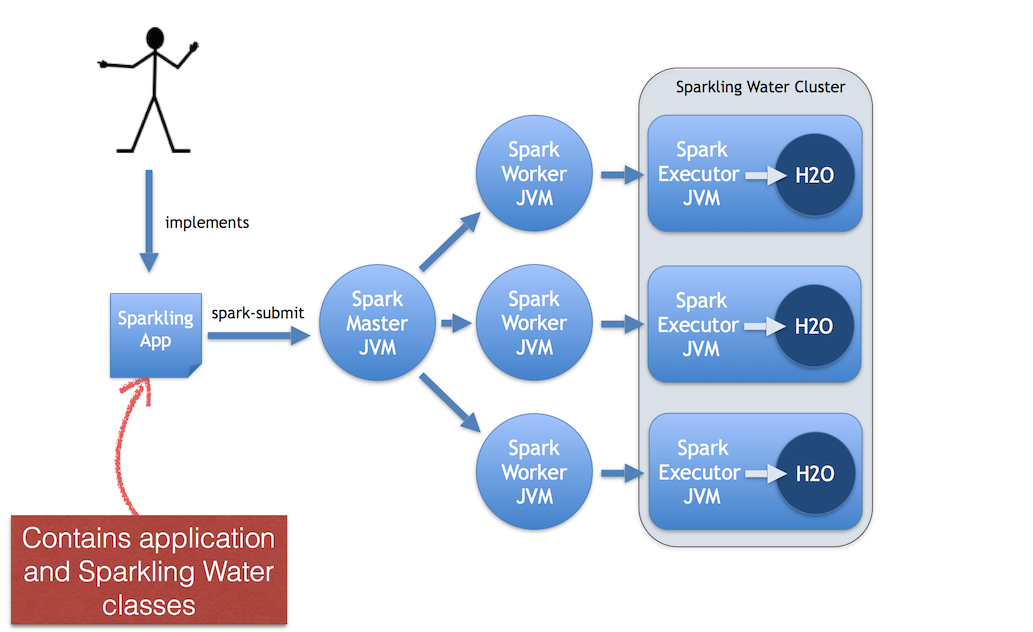
\includegraphics[scale=0.6]{sw/images/Topology.png}
	\caption{Sparkling Water design depicting deployment of the Sparkling Water application to the standalone Spark cluster.}
\end{figure}


\subsection{Data Sharing between Spark and H2O}

Sparkling Water enables transformation between different types of RDDs and H2O's \texttt{H2OFrame}, and vice versa.

When converting from an \texttt{H2OFrame} to an RDD, a wrapper is created around the \texttt{H2OFrame} to provide an RDD-like API. In this case,  data is not duplicated but served directly from the underlying \texttt{H2OFrame}.

Converting from an RDD/DataFrame to an \texttt{H2OFrame} requires data duplication because it transfers data from the RDD storage into \texttt{H2OFrame}. However, data stored in an \texttt{H2OFrame} is heavily compressed and does not need to be preserved in RDD.

\begin{figure}[h!]
	\centering
	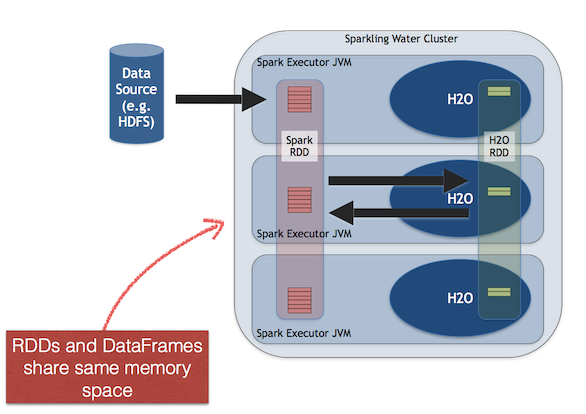
\includegraphics[scale=1]{sw/images/DataShare.png}
	\caption{Sharing between Spark and H2O inside an executor JVM.}
\end{figure}


\subsection{Provided Primitives}

Sparkling Water provides several primitives (for more information, refer to Table~\ref{tab:primitives}). Before using H2O algorithms and data structures, the first step is to create and start the \texttt{H2OContext} instance using the \texttt{val hc = new H2OContext(sc).start()} call. 

The \texttt{H2OContext} contains the necessary information for running H2O services and exposes methods for data transformation between the Spark RDD or \texttt{DataFrame} and the \texttt{H2OFrame}. Starting \texttt{H2OContext} involves a distributed operation that contacts all accessible Spark executor nodes and initializes H2O services (such as the key-value store and RPC) inside the executors' JVMs.

When \texttt{H2OContext} is running, H2O data structures and algorithms can be manipulated. The key data structure is \texttt{H2OFrame}, which represents a distributed table composed of vectors. A new \texttt{H2OFrame} can be created using one of the following methods:
\begin{itemize}
	\item loading a cluster local file (a file located on each node of the cluster):
\begin{lstlisting}[style=Scala]
val h2oFrame = new H2OFrame(new File("/data/iris.csv"))
\end{lstlisting}
	\item loading a file from HDFS/S3/S3N/S3A:
\begin{lstlisting}[style=Scala]
val h2oFrame = new H2OFrame(URI.create("hdfs://data/iris.csv"))
\end{lstlisting}
	\item loading multiple files from HDFS/S3/S3N/S3A:
\begin{lstlisting}[style=Scala]
val h2oFrame = new H2OFrame(URI.create("hdfs://data/iris/01.csv"), URI.create("hdfs://data/iris/02.csv"))
\end{lstlisting}
	\item transforming Spark RDD or \texttt{DataFrame}:
\begin{lstlisting}[style=Scala]
val h2oFrame = h2oContext.asH2OFrame(rdd)
\end{lstlisting}
	\item referencing existing \texttt{H2OFrame} by its key
\begin{lstlisting}[style=Scala]
val h2oFrame = new H2OFrame("iris.hex")
\end{lstlisting}		
\end{itemize}

\begin{table}[!ht]
\centering
%\begin{adjustbox}{width=\textwidth} %resizes table to text width
%\setlength{\tabcolsep}{2pt} %narrow column separation
\begin{tabular}{c c p{5.2cm}}
%\begin{tabularx}{\textwidth}{l l p{5.2cm}}
\toprule
Concept & API Representation & Description \\
\midrule
H2O Context & \texttt{H2OContext} & Contains
H2O state, provides primitives to publish \texttt{RDD} as \texttt{H2OFrame} and
vice versa. Follows design principles of Spark primitives such as
\texttt{SparkContext} or \texttt{SQLContext}. \\ \addlinespace
%\small{(Full name: \small{\texttt{org.apache.spark.\break h2o.H2OContext}}}) \\  \addlinespace

H2O Entry Point & \texttt{water.H2O} & Represents the entry point for accessing
H2O services. Contains information about running H2O services, including a list of
nodes and the status of the distributed K/V datastore. \\  \addlinespace

H2O Frame &  \small{\texttt{water.fvec.H2OFrame}} & A data structure 
representing a table of values. The table is column-based and provides column and
row accessors. \\  \addlinespace

H2O Algorithm & package \texttt{hex} & Represents the H2O machine learning
algorithms library, including DeepLearning, GBM, GLM, DRF, and other
algorithms. \\

\bottomrule
\end{tabular} 
%\end{tabularx}
\caption{Sparkling Water primitives}
\label{tab:primitives}
\end{table}

\pagebreak
When the \texttt{H2OContext} is running, any H2O algorithm can be called. Most of provided algorithms are located in the \texttt{hex} package. Calling an algorithm is composed of two steps:

\begin{itemize}
	\item Specifying parameters:
\begin{lstlisting}[style=Scala]
val train: H2OFrame = new H2OFrame(new File("prostate.csv"))
val gbmParams = new GBMParameters()
gbmParams._train = train
gbmParams._response_column = 'CAPSULE
gbmParams._ntrees = 10
\end{lstlisting}

	\item Creating the model builder and launching computations. The \texttt{trainModel} method is non-blocking and returns a job representing the computation.
\begin{lstlisting}[style=Scala]
val gbmModel = new GBM(gbmParams).trainModel.get
\end{lstlisting}
\end{itemize}

\end{document}

%
% Exposed public Scala API
%
\newpage
\section{Programming API}

\subsection{Starting H2O Services}

\begin{lstlisting}[style=Scala]
val sc: SparkContext = ...
val hc = H2OContext.getOrCreate(sc)
\end{lstlisting} 
or:
\begin{lstlisting}[style=Scala]
val sc: SparkContext = ...
val hc = new H2OContext(sc).start()
\end{lstlisting}

When the number of Spark nodes is known, it can be specified in the \texttt{getOrCreate} call:

\begin{lstlisting}[style=Scala]
val hc = H2OContext.getOrCreate(sc, numOfSparkNodes)
\end{lstlisting}
or, in start method of \texttt{H2OContext}:

\begin{lstlisting}[style=Scala]
val hc = new H2OContext(sc).start(numOfSparkNodes)
\end{lstlisting}

The former variant is preferred, because it initiates and starts \texttt{H2OContext} in one call and can be used to obtain already existing \texttt{H2OContext}. It is semantically the same as the latter variant though.

\subsection{Memory Allocation}

H2O resides in the same executor JVM as Spark. The memory provided for H2O is configured via Spark; refer to Spark configuration for more details.

\textbf{Generic configuration}

\begin{itemize}
\item Configure the Executor memory (i.e., memory available for H2O) via the Spark configuration property \texttt{spark.executor.memory}. For example, {\lstinline[style=Bash]|bin/sparkling-shell --conf spark.executor.memory=5g|} or configure the property in {\lstinline[style=Bash]|$SPARK_HOME/conf/spark-defaults.conf|}
\item Configure the Driver memory (i.e., memory available for H2O client running inside the Spark driver) via the Spark configuration property \texttt{spark.driver.memory}. For example, {\lstinline[style=Bash]|bin/sparkling-shell --conf spark.driver.memory=4g|} or configure the property in {\lstinline[style=Bash]|$SPARK_HOME/conf/spark-defaults.conf|}.
\end{itemize}

\pagebreak
\textbf{Yarn specific configuration}

\begin{itemize}
\item Refer to the Spark documentation \url{https://spark.apache.org/docs/latest/running-on-yarn.html}
\item For JVMs that require a large amount of memory, we strongly recommend configuring the maximum amount of memory available for individual mappers.
 \end{itemize} 
 
 \subsection{Converting H2OFrame into RDD[T]}
 
 The \texttt{H2OContext} class provides the explicit conversion, \texttt{asRDD}, which creates an RDD-like wrapper around the provided \texttt{H2OFrame}:

\begin{lstlisting}[style=Scala]
def asRDD[A <: Product: TypeTag: ClassTag](fr: H2OFrame): RDD[A]
\end{lstlisting}

The call expects the type \texttt{A} to create a correctly-typed RDD. The conversion requires type \texttt{A} to be bound by \texttt{Product} interface. The relationship between the columns of \texttt{H2OFrame} and the attributes of class \texttt{A} is based on name matching.

\textbf{Example}

\begin{lstlisting}[style=Scala]
val df: H2OFrame = ...
val rdd = asRDD[Weather](df)
\end{lstlisting}

\subsection{Converting H2OFrame into DataFrame}

The \texttt{H2OContext} class provides the explicit conversion, \texttt{asDataFrame}, which creates a \texttt{DataFrame}-like wrapper around the provided \texttt{H2OFrame}. Technically, it provides the \texttt{RDD[sql.Row]} RDD API:

\begin{lstlisting}[style=Scala]
def asDataFrame(fr: H2OFrame)(implicit sqlContext: SQLContext): DataFrame
\end{lstlisting}

This call does not require any type of parameters, but since it creates \texttt{DataFrame} instances, it requires access to an instance of \texttt{SQLContext}. In this case, the instance is provided as an implicit parameter of the call. The parameter can be passed in two ways: as an explicit parameter or by introducing an implicit variable into the current context.

The schema of the created instance of the \texttt{DataFrame} is derived from the column name and the types of \texttt{H2OFrame} specified.

\textbf{Example}

Using an explicit parameter in the call to pass \texttt{sqlContext}:

\begin{lstlisting}[style=Scala]
val sqlContext = new SQLContext(sc)
val schemaRDD = asDataFrame(h2oFrame)(sqlContext)
\end{lstlisting}

or as implicit variable provided by actual environment:

\begin{lstlisting}[style=Scala]
implicit val sqlContext = new SQLContext(sc)
val schemaRDD = asDataFrame(h2oFrame)
\end{lstlisting}

\subsection{Converting RDD[T] into H2OFrame}

The \texttt{H2OContext} provides implicit conversion from the specified \texttt{RDD[A]} to \texttt{H2OFrame}. As with conversion in the opposite direction, the type \texttt{A} has to satisfy the upper bound expressed by the type \texttt{Product}. The conversion will create a new \texttt{H2OFrame}, transfer data from the specified RDD, and save it to the H2O K/V data store.

\begin{lstlisting}[style=Scala]
implicit def asH2OFrame[A <: Product: TypeTag](rdd: RDD[A]): H2OFrame
\end{lstlisting}

The API also provides explicit version which allows for specifying name for resulting \texttt{H2OFrame}.

\begin{lstlisting}[style=Scala]
def asH2OFrame[A <: Product: TypeTag](rdd: RDD[A], frameName: String): H2OFrame
\end{lstlisting}

\textbf{Example}

\begin{lstlisting}[style=Scala]
val rdd: RDD[Weather] = ...
import h2oContext._
// Implicit call of H2OContext.asH2OFrame[Weather](rdd) is used 
val hf: H2OFrame = rdd
// Explicit call of of H2OContext API with name for resulting H2OFrame
val hfNamed: H2OFrame = h2oContext.asH2OFrame(rdd, "hfNamed")
\end{lstlisting}

\subsection{Converting DataFrame into H2OFrame}

The \texttt{H2OContext} provides \textbf{implicit} conversion from the specified \texttt{DataFrame} to \texttt{H2OFrame}. The conversion will create a new \texttt{H2OFrame}, transfer data from the specified \texttt{DataFrame}, and save it to the H2O K/V data store.

\begin{lstlisting}[style=Scala]
implicit def asH2OFrame(rdd: DataFrame): H2OFrame
\end{lstlisting}

The API also provides explicit version which allows for specifying name for resulting \texttt{H2OFrame}.

\begin{lstlisting}[style=Scala]
def asH2OFrame(rdd: DataFrame, frameName: String): H2OFrame
\end{lstlisting}

\textbf{Example}

\begin{lstlisting}[style=Scala]
val df: DataFrame = ...
import h2oContext._
// Implicit call of H2OContext.asH2OFrame(srdd) is used 
val hf: H2OFrame = df 
// Explicit call of H2Context API with name for resulting H2OFrame
val hfNamed: H2OFrame = h2oContext.asH2OFrame(df, "hfNamed")
\end{lstlisting}

\subsection{Creating H2OFrame from an Existing Key}

If the H2O cluster already contains a loaded \texttt{H2OFrame} referenced by the key \texttt{train.hex}, it is possible to reference it from Sparkling Water by creating a proxy \texttt{H2OFrame} instance using the key as the input:

\begin{lstlisting}[style=Scala]
val trainHF = new H2OFrame("train.hex")
\end{lstlisting}

\subsection{Type Map Between H2OFrame and Spark DataFrame Types}

For all primitive Scala types or Spark SQL types (see \linebreak \texttt{org.apache.spark.sql.types}) which can be part of Spark RDD/DataFrame, we provide mapping into H2O vector types (numeric, categorical, string, time, UUID - see \texttt{water.fvec.Vec}):

\begin{table}[!ht]
\centering
\begin{tabular}{l l l}
\toprule
Scala type  &	SQL type 	& H2O type \\
\midrule
NA & BinaryType & Numeric \\
Byte 	& ByteType & Numeric \\
Short & ShortType & Numeric \\
Integer & IntegerType & Numeric \\
Long & LongType & Numeric \\
Float & FloatType & Numeric \\
Double & DoubleType & Numeric \\
String & StringType & String \\
Boolean & BooleanType & Numeric \\
java.sql.TimeStamp & TimestampType & Time \\
\bottomrule
\end{tabular} 
\end{table}

\subsection{Calling H2O Algorithms}

\begin{enumerate}
\item Create the parameters object that holds references to input data and parameters specific for the algorithm:

\begin{lstlisting}[style=Scala]
val train: RDD = ...
val valid: H2OFrame = ...

val gbmParams = new GBMParameters()
gbmParams._train = train
gbmParams._valid = valid
gbmParams._response_column = 'bikes
gbmParams._ntrees = 500
gbmParams._max_depth = 6
\end{lstlisting}

 \item Create a model builder:
 \begin{lstlisting}[style=Scala]
 val gbm = new GBM(gbmParams)
 \end{lstlisting}
 
 \item Invoke the model build job and block until the end of computation (\texttt{trainModel} is an asynchronous call by default): 
 \begin{lstlisting}[style=Scala]
 val gbmModel = gbm.trainModel.get 
 \end{lstlisting}
 \end{enumerate}

\subsection{Using Spark Data Sources with H2OFrame}
Spark SQL provides configurable data source for SQL tables. Sparkling Water enable \texttt{H2OFrame} to be
used as data source to load/save data from/to Spark SQL table.

\subsubsection{Reading from \texttt{H2OFrame}}

Let's suppose we have a \texttt{H2OFrame}. The shortest way to load a \texttt{DataFrame} from \texttt{H2OFrame} with default settings is:
\begin{lstlisting}[style=Scala]
val df = sqlContext.read.h2o(frame.key)
\end{lstlisting}

There are two more ways to load a \texttt{DataFrame} from \texttt{H2OFrame} allowing us to specify additional options:
\begin{lstlisting}[style=Scala]
val df = sqlContext.read.format("h2o").option("key",frame.key.toString).load()
\end{lstlisting}
or
\begin{lstlisting}[style=Scala]
val df = sqlContext.read.format("h2o").load(frame.key.toString)
\end{lstlisting}

\subsubsection{Saving to \texttt{H2OFrame}}

Let's suppose we have \texttt{DataFrame} df. The shortest way to save the \texttt{DataFrame} as \texttt{H2OFrame} with default settings is:
\begin{lstlisting}[style=Scala]
df.write.h2o("new_key")
\end{lstlisting}

There are two more ways to save the \texttt{DataFrame} as \texttt{H2OFrame} allowing us to specify additional options:
\begin{lstlisting}[style=Scala]
df.write.format("h2o").option("key","new_key").save()
\end{lstlisting}
or
\begin{lstlisting}[style=Scala]
df.write.format("h2o").save("new_key")
\end{lstlisting}

All three variants save the \texttt{DataFrame} as \texttt{H2OFrame} with the key "new\_key". They won't succeed if a \texttt{H2OFrame} with the same key already exists.

\subsubsection{Loading and Saving Options}

If the key is specified as 'key' option, and also in the load/save method, the option 'key' is preferred:
\begin{lstlisting}[style=Scala]
val df = sqlContext.read.from("h2o").option("key","key_one").load("key_two")
\end{lstlisting}
or
\begin{lstlisting}[style=Scala]
val df = sqlContext.read.from("h2o").option("key","key_one").save("key_two")
\end{lstlisting}

In both examples, "key\_one" is used.

\subsubsection{Specifying Saving Mode}

There are four save modes available when saving data using Data Source API- see \url{http://spark.apache.org/docs/latest/sql-programming-guide.html#save-modes}

\begin{itemize}
\item If "append" mode is used, an existing \texttt{H2OFrame} with the same key is deleted, and a new one created with the same key. The new frame contains the union of all rows from the original \texttt{H2OFrame} and the appended \texttt{DataFrame}.
\item If "overwrite" mode is used, an existing \texttt{H2OFrame} with the same key is deleted, and new one with the new rows is created with the same key.
\item If "error" mode is used, and a \texttt{H2OFrame} with the specified key already exists, an exception is thrown.
\item If "ignore" mode is used, and a \texttt{H2OFrame} with the specified key already exists, no data are changed.
\end{itemize}

%
% Building standalone applications with Sparklint Water
%
\newpage
\section{Building a Standalone Application}

\textbf{Sparkling Water Example Project}

This is a structure of a simple example project to start coding with Sparkling Water. The source code is available at
\url{https://github.com/h2oai/h2o-droplets/tree/master/sparkling-water-droplet}

\textbf{Dependencies}

This droplet uses Sparkling Water 2.2, which integrates:
\begin{itemize}
\item Spark 2.2
\item H2O 3.14.0.7 Weierstrass
\end{itemize}

For more details see \texttt{build.gradle}.

\textbf{Project structure}

% Lots of code to draw a basic file structure, examples exist to jazz this up
\begin{forest}
  for tree={
    %font=\ttfamily,
    grow'=0,
    child anchor=west,
    parent anchor=south,
    anchor=west,
    calign=first,
    edge path={
      \noexpand\path [draw, \forestoption{edge}]
      (!u.south west) +(7.5pt,0) |- node[fill,inner sep=1.25pt] {} (.child anchor)\forestoption{edge label};
    },
    before typesetting nodes={
      if n=1
        {insert before={[,phantom]}}
        {}
    },
    fit=band,
    before computing xy={l=15pt},
  }
[
  [\texttt{gradle/} ........ Gradle definition files]
  [\texttt{src/} .............. Source code
    [\texttt{main/} ....... Main implementation code
      [\texttt{scala/} ]
    ]
    [\texttt{test/} ....... Test code
      [\texttt{scala/}]
    ]
  ]
  [\texttt{build.gradle} ... Build file for this project]
  [\texttt{gradlew} ........ Gradle wrapper]
]
\end{forest}

\textbf{Project building}

For building, please, use provided gradlew command:

\begin{lstlisting}[style=Bash]
./gradlew build
\end{lstlisting}

\textbf{Run demo}

For running a simple application:

\begin{lstlisting}[style=Bash]
./gradlew run
\end{lstlisting}

\textbf{Starting with IDEA}

There are two ways to open this project in IntelliJ IDEA

Using Gradle build file directly:

\quad Open the project's \texttt{build.gradle} in IDEA via File $\rightarrow$ Open

or using Gradle generated project files:

\begin{enumerate}
\item Generate Idea configuration files via  {\lstinline[style=Bash]|./gradlew idea|} 
\item Open project in Idea via File $\rightarrow$ Open
\end{enumerate}

Note: To clean up Idea project files please launch {\lstinline[style=Bash]|./gradlew cleanIdea|} 

\textbf{Starting with Eclipse}

\begin{enumerate}
\item Generate Eclipse project files via {\lstinline[style=Bash]|./gradlew eclipse|} 
\item Open project in Eclipse via File $\rightarrow$ Import $\rightarrow$ Existing Projects into Workspace
\end{enumerate}

\textbf{Running tests}

To run tests, please, run:

\begin{lstlisting}[style=Bash]
./gradlew test
\end{lstlisting}

\textbf{Checking code style}

To check codestyle:

\begin{lstlisting}[style=Bash]
./gradlew scalaStyle
\end{lstlisting}

\textbf{Creating and Running Spark Application}

Create application assembly which can be directly submitted to Spark cluster:

\begin{lstlisting}[style=Bash]
./gradlew shadowJar
\end{lstlisting}

The command creates jar file \texttt{build/libs/sparkling-water-droplet-}\\
\texttt{app.jar} containing all necessary classes to run application on top of Spark cluster.

Submit application to Spark cluster (in this case, local cluster is used):

\begin{lstlisting}[style=Bash]
export MASTER="local[*]"
$SPARK_HOME/bin/spark-submit --class water.droplets.SparklingWaterDroplet build/libs/sparkling-water-droplet-all.jar
\end{lstlisting}




\newpage
\section{Appendix A: Complete parameter list}


\newpage
\section{Appendix B: References}

\end{document}

